\documentclass[a4paper,11pt]{article}
\usepackage[left=1.5cm,right=1.5cm,top=2.0cm,bottom=2.8cm]{geometry}

\usepackage[ngerman,american]{babel}
\usepackage{graphicx}
\usepackage{amsmath}
\usepackage{amsthm}
\usepackage{amssymb}
\usepackage{listings}
\usepackage{epstopdf}
\usepackage{sidecap}
% \usepackage[FIGTOPCAP]{subfigure}
\usepackage{float}
\usepackage{color}
\usepackage[usenames,dvipsnames]{xcolor}
%\usepackage{empheq}
\usepackage[footnotesize,bf]{caption}
\usepackage{subcaption}
%\usepackage[framed,numbered,autolinebreaks,useliterate]{mcode}
\usepackage[utf8x]{inputenc}
\usepackage{lmodern, textcomp}


\theoremstyle{definition}
\newtheorem{defi}{Definition}
\theoremstyle{plain}
\newtheorem{theo}[defi]{Theorem}
\theoremstyle{remark}
\newtheorem{remark}{Remark}

\providecommand{\abs}[1]{\lvert#1\rvert}
\providecommand{\norm}[1]{\lVert#1\rVert}

\renewcommand{\vec}[1]{\boldsymbol{#1}}

\title{Exercise 11}
\author{Philipp Hanslovsky, Robert Walecki}

\begin{document}


\lstloadlanguages{R} 
\lstset{language=R,
   %keywords={break,case,catch,continue,else,elseif,end,for,function,
   %   global,if,otherwise,persistent,return,switch,try,while},
   basicstyle=\ttfamily,
   keywordstyle=\color{blue},
   commentstyle=\color{green!40!black},
   stringstyle=\color{red},
   numbers=left,
   numberstyle=\tiny\color{white!50!black},
   stepnumber=1,
   numbersep=10pt,
   backgroundcolor=\color{white},
   tabsize=4,
   showspaces=false,
   showstringspaces=false,
   frame=single}

\def\dblone{\hbox{$1\hskip -1.2pt\vrule depth 0pt height 1.6ex width 0.7pt
                  \vrule depth 0pt height 0.3pt width 0.12em$}}

\maketitle

\section*{11.1.1}
The question can be formulated as a LP:
\begin{flalign}
&\operatorname*{arg\,max}_x c^Tx \\
&s.t. \\
&e^Tx = 40 \\
&x \le d\\
&x = (x1, x2)^T, c = (2.5, 3.0)^T, e = (1/2, 1/1.4)^T, d = (60, 40)^T 
\end{flalign}
$x$ is the amount of cherries and apples plucked. $c$ is the profit. $e$ is the effort to pluck 1kg. $d$ is the maximum demand.

\section*{11.1.2}
The optimal solution is selling 60kg of cherries and 14kg of apples. The profit then amounts to 192€.

\section*{11.1.3}
The dual is derived from the Lagrangian:
\begin{flalign}
&g(\lambda, \nu) = \sup_xL(x,\lambda,\nu) \\
&\mathcal{L} = c^Tx +\lambda^T(d-x) + \nu(e^Tx - 40) = x^T(c-\lambda+\nu e)+\lambda^Td-40\nu, \lambda \ge 0 \\
&g(\lambda, \nu) = \begin{cases}
                   \lambda^Td - 40 \nu & (c - \lambda + \nu e) = 0 \\
                   -\infty & {\text otherwise}
                   \end{cases}
\end{flalign}

It is obvious that the infinite infimum is not of any use. The dual problem is the minimization of $g$:

\begin{flalign}
&\operatorname*{arg\,min}_{\lambda, \nu} d^T\lambda - 40 \nu \\
&s.t. \\
&c-\lambda+\nu e = 0 \\
&\lambda \ge 0
\end{flalign}

The dual of the dual can be derived the same way:
\begin{flalign}
&\mathcal{L} = d^T\lambda-40\nu+k^T(c-\lambda+\nu e)-l^T\lambda = \lambda^T(d-k-l)+\nu(-40+e^Tk), l \ge 0 \\
&\operatorname*{arg\,max}_k g = \operatorname*{arg\,max}_k \inf_{\lambda,\nu}L = \operatorname*{arg\,max}_k c^Tk \\
&s.t. \\
&k-d \le 0\\
&e^Tk = 0
\end{flalign}
Comparing the dual of the dual with the primal it becomes obvious that $k=x$ and the dual of the dual is the primal.
Note: In order to minimize the primal and to maximize the dual, it is neccessary to multiply both problems with $-1$. That does not change a

\section*{11.2.1}
The least squares method does not fit the data very well. The outliers distort the data resulting in a too steep slope (see fig. \ref{fig:regress}).
\begin{figure}[H]
\centering
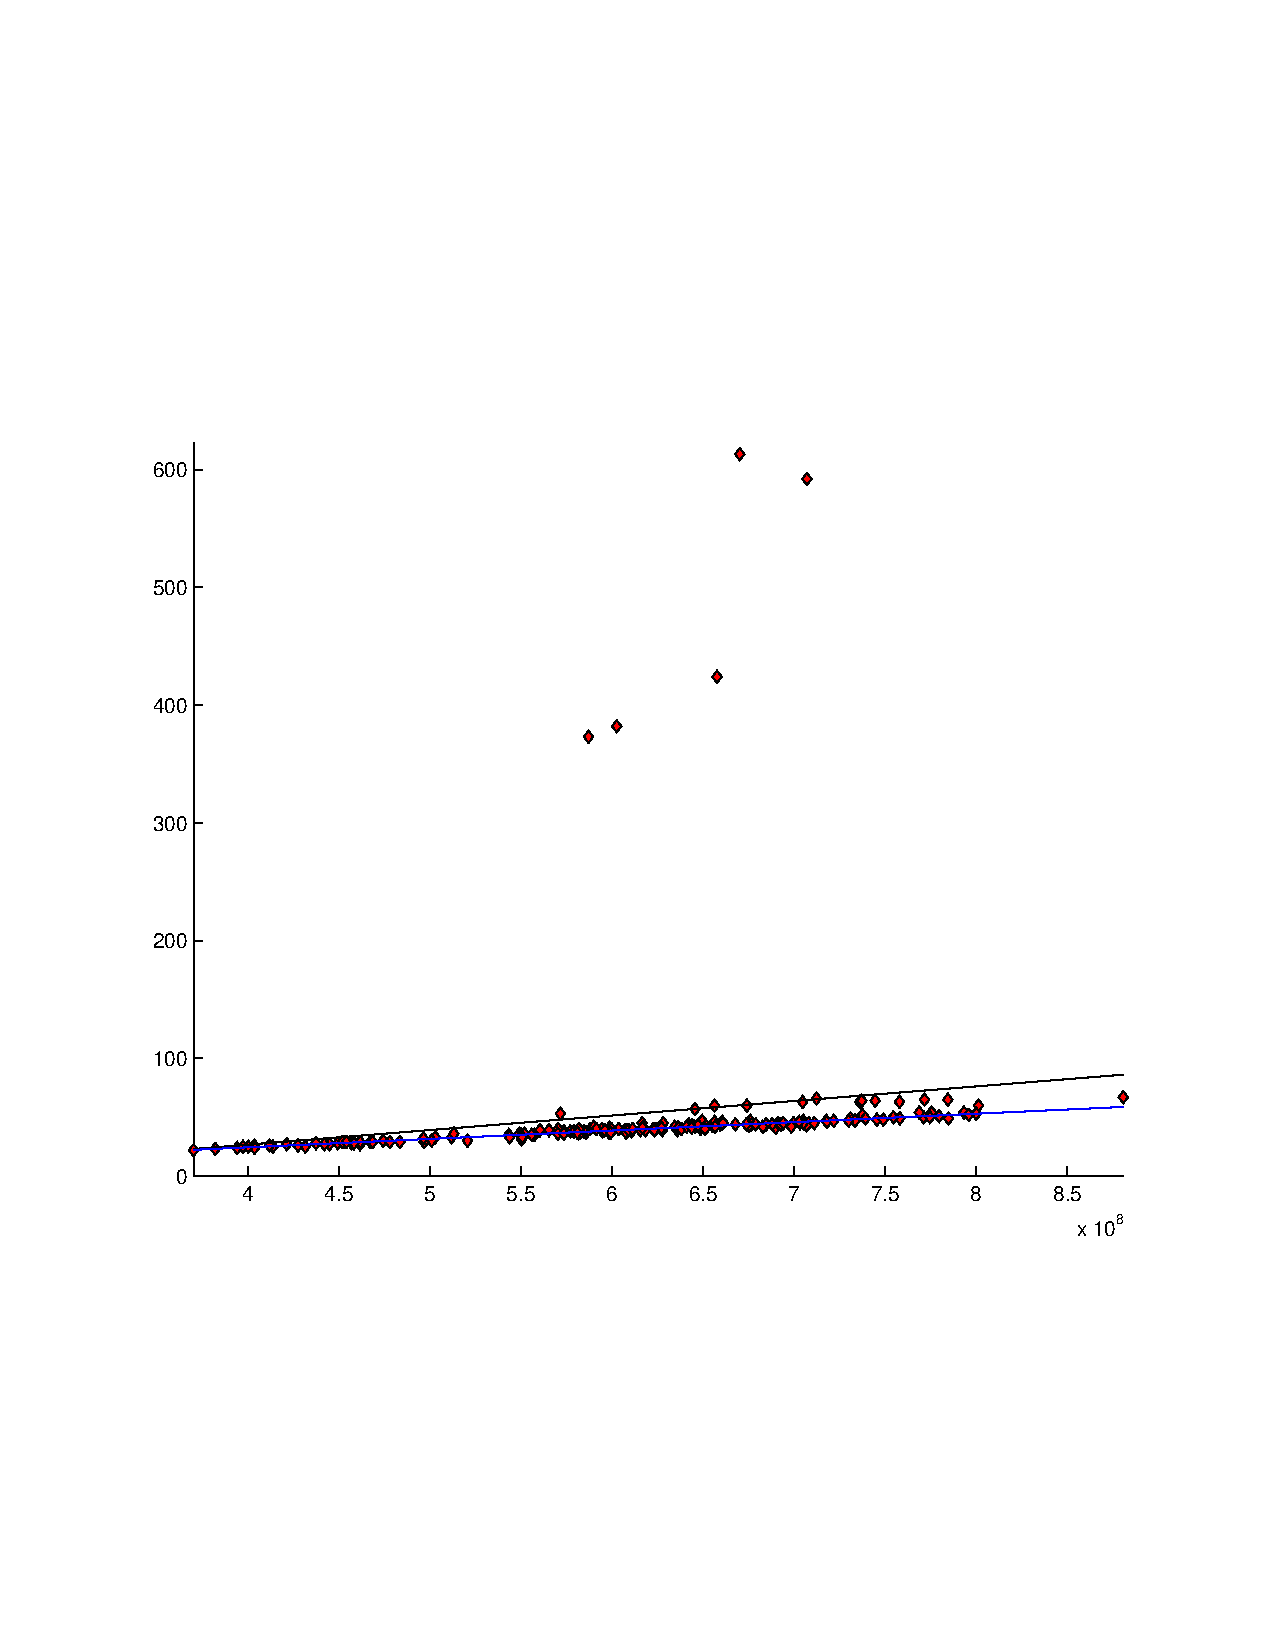
\includegraphics[width=0.7\textwidth]{regression.pdf}
\caption{data and fits for different regression methods}
\label{fig:regress}
\end{figure}

\section*{11.2.2}
\begin{flalign}
&\hat{x} = \operatorname*{arg\,min}_x ||y-Ax|| = \operatorname*{arg\,min}_x\sum_i|y_i-\sum_ja_{ij}x_j|
\end{flalign}
$y$ contains the observed values at coordinates given by $A$. $x$ are the regression parameters to be optimized. This problem can be translated to a linear program:
\begin{flalign}
&\hat{x} = \operatorname*{arg\,min}_{v,x} \mathbb{I}^Tv \\
& s.t. \\
-&v + Ax \le y \\
-&v - Ax \le y
\end{flalign}
$\mathbb{I}$ is a vector of ones of the same dimension as $v$. 
This can be rewritten as:
\begin{flalign}
&\operatorname*{arg\,min}_{\tilde{x}} c^T\tilde{x} \\
&s.t. \\
&\tilde{A}\tilde{x} \le \tilde{y} \\
&\tilde{A} = \begin{pmatrix}
            A & - \dblone \\
            -A & -\dblone
            \end{pmatrix},
\tilde{x} = (x, v)^T, \tilde{y} = (y, -y)^T, c = (0, \mathbb{I})^T
\end{flalign}
$\dblone$ is the identity matrix, the others as before.

\section*{11.2.3}
The $L_1$ fit is more robust against outliers. The line is closer to the points that are actual data and not outliers (see fig. \ref{fig:regress}). With least squares larger distances (i.e. outliers) are weighted more strongly.

\end{document}
